\begin{frame}
    \frametitle{ADC}
    
    \begin{figure}
        \centering
        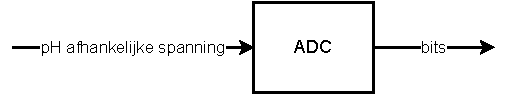
\includegraphics[width=\textwidth]{adcBlock}
    \end{figure}

\end{frame}

\begin{frame}
    \frametitle{Eisen}

    \begin{table}[ht]
        \centering
        \begin{tabular}{l|c|l}
            Symbol      & Waarde & Eenheid\\\hline
            $SNR_{in}$  & 37        & dB\\
            NF          & 3         & dB\\
            $u_{in}$    & 2.5       & mV\\
        \end{tabular}
        \caption{De eisen voor het omzetten van het analoge signaal naar een digitaal signaal.}
        \label{tab:systemSpecADC}
    \end{table}
    
\end{frame}
\begin{frame}
    \frametitle{Minimum aantal bits}
    \centering

    De toelaatbare fout ten gevolge van de eindige resolutie van de ADC
    \begin{equation*}\label{eq:calcSpecifiedRmsError}
        \overline{e_{eff}^2}=\left(10^{\frac{NF}{10}}-1\right)\left(\frac{S_{rms}}{10^{\left(SNR+NF\right)/20}}\right)^2
    \end{equation*}
    \pause


    Berekenen minimum benodigde ADC resolutie
    \begin{equation*}\label{eq:calcNeededQ}
        Q=\sqrt{12\cdot\overline{e_{eff}^2}}
    \end{equation*}
    \pause

    Berekenen minimum aantal bits van de ADC op basis van de minimaal benodigde ADC resolutie 
    \begin{equation*}\label{eq:calcMinNumberADCbits}
        n=\left\lceil\log_2\left(\frac{1}{Q}+1\right)\right\rceil=14
    \end{equation*}

\end{frame}

\begin{frame}
    \frametitle{Sample frequentie}
    \centering
    
    Toelaatbare fout
    \begin{equation*}\label{eq:ADCmaxSampleError}
        E=10^{\frac{-NF}{10}}
    \end{equation*}
    \pause

    Minimale sample frequentie
    \begin{equation*}\label{eq:ADCminFs}
        f_{s,min}=\frac{\pi f_h}{E}= \qty{45}{\hertz}
    \end{equation*}

\end{frame}
